\begin{tcolorbox}[title=Definition: Logic circuit (digital circuit)]
Receives input signals $p_1, p_2,\ldots, p_n$, each a bit [either 0 (off) or 1 (on)], and produces output signals $s_1, s_2,\ldots, s_n$, each a bit.  
\end{tcolorbox}
\begin{tcolorbox}[colback=white, colframe=gray!60, title=Remark 1]
In this section we will
restrict our attention to logic circuits with a single output signal; in general, digital circuits may
have multiple outputs.
\end{tcolorbox}
\begin{tcolorbox}[title=Definition: Basic Logic Gates]
Complicated digital circuits can be constructed from three basic circuits, called gates:

\begin{enumerate}
    \item The \textbf{inverter}, or \textbf{NOT gate}, takes an input bit $p$ and produces as output $\neg p$.
\begin{center}
    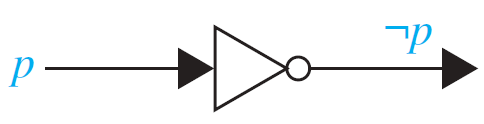
\includegraphics[width=0.3\linewidth]{chp1_2_applogic/inv.png}
\end{center}
    \item The \textbf{OR gate} takes two input signals $p$ and $q$, each a bit, and produces as output the signal $p\lor q$.
\begin{center}
    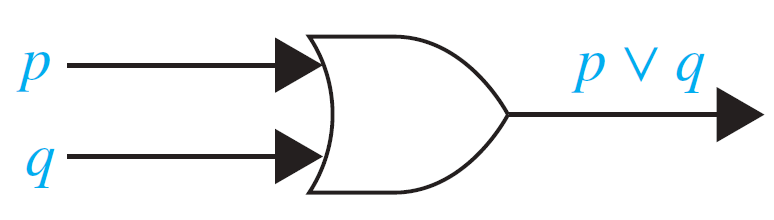
\includegraphics[width=0.3\linewidth]{chp1_2_applogic/or.png}
\end{center}
    \item The \textbf{AND gate} takes two input signals $p$ and $q$, each a bit, and produces as output the signal $p\land q$.
\begin{center}
    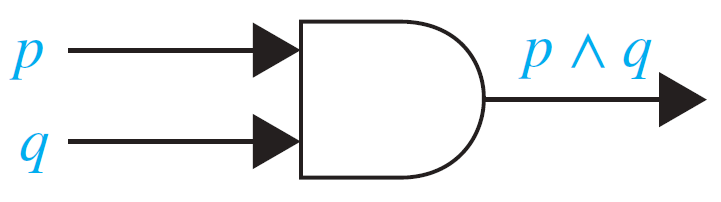
\includegraphics[width=0.3\linewidth]{chp1_2_applogic/and.png}
\end{center}
\end{enumerate}
\end{tcolorbox}

\begin{tcolorbox}[title=Example 1: Output for the combinatorial circuit]
Determine the output for the combinatorial circuit
\begin{center}
    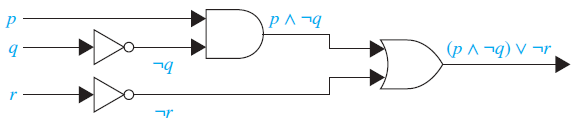
\includegraphics[width=0.6\linewidth]{chp1_2_applogic/comb1.png}
\end{center}
\textbf{Strategy:}
We display the output of each logic gate in the circuit
\begin{itemize}
    \item We see that the \textbf{AND gate} takes input of $p$ and $\neg q$, the output of the inverter with input $q$, and produces $p \land \neg q$
    \item Next, we note that the \textbf{OR gate} takes input $p \land \neg q$ and $\neg r$ (the output of the inverter with
input $r$), and produces the final output $(p \land \neg q) \lor \neg r$ .
\end{itemize}
\end{tcolorbox}
\begin{tcolorbox}[title=Example 2: Combinatorial circuit when want a certain output]
Build a digital circuit that produces the output 
\begin{center}
$\left(p \lor \neg r \right) \land \left(\neg p \lor (q \lor \neg r) \right)$    
\end{center}
when given input bits $p$, $q$, and $r$. \\ \\
\textbf{Strategy:}
We start with the output and "work backwards"
\begin{itemize}
    \item \textbf{Output}: $\left(p \lor \neg r \right) \land \left(\neg p \lor (q \lor \neg r) \right)$ is a conjunction (\textbf{AND gate}) between $\left(p \lor \neg r \right)$ and $\left(\neg p \lor (q \lor \neg r) \right)$
    \item $\mathbf{p \lor \neg r }$ : This is a disjunction (\textbf{OR gate}) between $p$ and $\neg r$
    \item $\mathbf{\neg r}$: This is a negation (\textbf{Inverter/NOT gate}) of $r$
    \item $\mathbf{\neg p \lor (q \lor \neg r) }:$ This is a disjunction (\textbf{OR gate}) between $\neg p$ and $q \lor \neg r$
    \item $\mathbf{\neg p}$: This is a negation (\textbf{Inverter/NOT gate}) of $p$
    \item $\mathbf{q \lor \neg r}:$ This is a disjunction between $q$ and $\neg r$
\end{itemize}
\textbf{Conclusion and figure:}
\begin{center}
    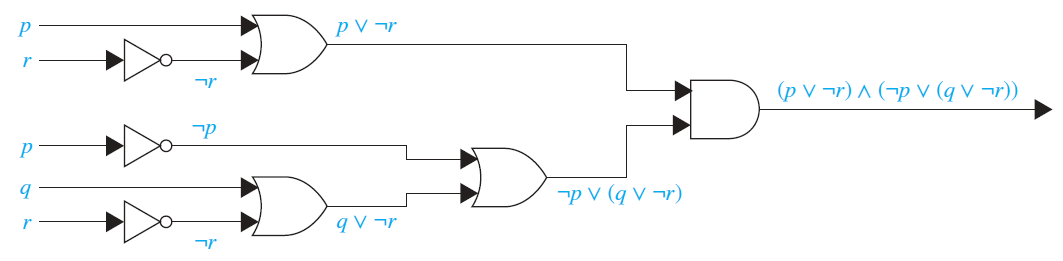
\includegraphics[width=0.9\linewidth]{chp1_2_applogic/comb2.png}
\end{center}
\end{tcolorbox}











